\subsection{UC8 - Impostazioni PCA}
    \label{uc8}
    
    \begin{figure}[htbp]
        \centering
        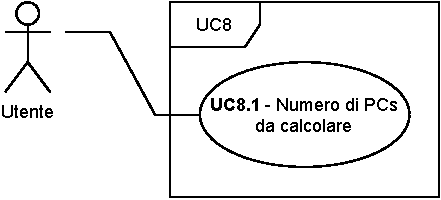
\includegraphics[width=0.5\textwidth]{source/sections/casi-uso/diagrams/uc8.pdf}
        \caption{UC8 - Impostazioni PCA}
        \label{fig:uc8}
    \end{figure}
    
    \begin{itemize}
    \item \textbf{Attore}: utente;
    \item \textbf{Descrizione}: l'utente specifica le impostazioni con cui l'algoritmo PCA calcolerà il risultato
    \item \textbf{Precondizione}: 
    \begin{itemize}
        \item eseguito l'upload del dataset come matrice $N\times M$ (\hyperref[uc1]{UC1});
        \item selezionato Linear Projection come visualizzazione (\hyperref[uc2.5]{UC2.5});
        \item selezionato PCA (\hyperref[uc7.1]{UC7.1}).
    \end{itemize}  
    \item \textbf{Postcondizione}: le impostazioni sono state definite come desiderato dall'utente
    \item \textbf{Scenario Principale}: 
    \begin{enumerate}
        \item l'utente specifica le impostazioni richieste dall'algoritmo
    \end{enumerate}  
    \end{itemize}
    
    
    \subsubsection{UC8.1 - Numero di PCs da calcolare}
    \label{uc8.1}
    \begin{itemize}
    \item \textbf{Attore}: utente;
    \item \textbf{Descrizione}: l'utente specifica quante nuove features il PCA deve calcolare;
    \item \textbf{Precondizione}: 
    \begin{itemize}
        \item eseguito l'upload del dataset come matrice $N\times M$ (\hyperref[uc1]{UC1});
        \item selezionato Linear Projection come visualizzazione (\hyperref[uc2.5]{UC2.5});
        \item selezionato PCA (\hyperref[uc7.1]{UC7.1}).
    \end{itemize}  
    \item \textbf{Postcondizione}: il numero k di features da calcolare è stato inserito;
    \item \textbf{Scenario Principale}: 
    \begin{enumerate}
        \item l'utente inserisce un numero k compreso tra 1 e il numero di features.
    \end{enumerate}  
    \end{itemize}